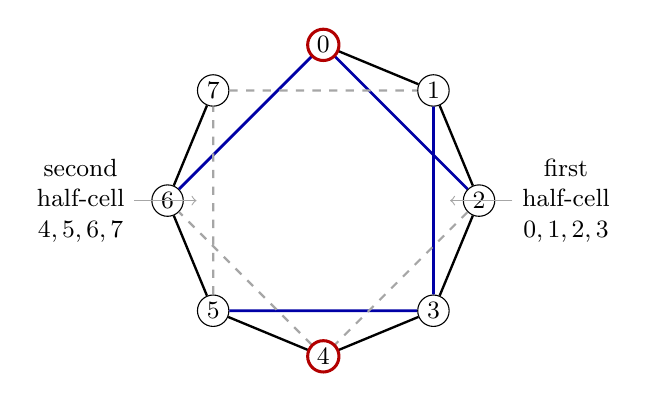
\begin{tikzpicture}[scale=0.92,
 vertex/.style={circle,draw,fill=white,inner sep=1.4pt,font=\small},
 defect/.style={circle,draw=red!70!black,line width=1.1pt,inner sep=4pt}]
 \node[vertex] (v0) at (90:2.15) {$0$};
 \node[vertex] (v1) at (45:2.15) {$1$};
 \node[vertex] (v2) at (0:2.15) {$2$};
 \node[vertex] (v3) at (-45:2.15) {$3$};
 \node[vertex] (v4) at (-90:2.15) {$4$};
 \node[vertex] (v5) at (-135:2.15) {$5$};
 \node[vertex] (v6) at (180:2.15) {$6$};
 \node[vertex] (v7) at (135:2.15) {$7$};
 \draw[line width=.85pt] (v0)--(v1)--(v2)--(v3)--(v4)--(v5)--(v6)--(v7)--cycle;
 \draw[blue!65!black,line width=1pt]
   (v0)--(v2) (v1)--(v3) (v3)--(v5) (v6)--(v0);
 \draw[gray!70,dashed,line width=.8pt]
   (v2)--(v4) (v4)--(v6) (v5)--(v7) (v7)--(v1);
 \node[defect] at (v0) {};
 \node[defect] at (v4) {};
 \node[font=\small,align=center] (hl) at (-3.35,0) {second\\half-cell\\$4,5,6,7$};
 \node[font=\small,align=center] (hr) at (3.35,0) {first\\half-cell\\$0,1,2,3$};
 \draw[->,gray!70] (hl.east)--(-1.75,0);
 \draw[->,gray!70] (hr.west)--(1.75,0);
\end{tikzpicture}
